% 0315(본책 50쪽) — 원 (x-3)^2+(y-1)^2=4 가 x축·직선 y=ax 와 만나서 생기는 길이가 같은 두 현. 스캔 그림이라 TikZ 로 다시 그림.
% 라벨은 원문 그대로 O·x·y·y=ax·원의 식과 두 현의 같음 표시(짧은 선)만. a 의 값(답)이 드러나지 않게 직선 기울기는 원문 모양대로 대략 그림.
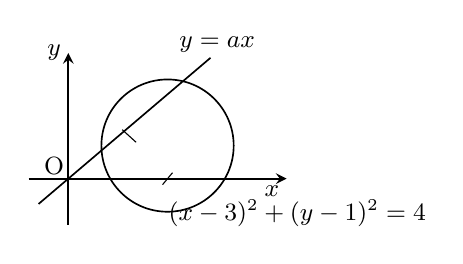
\begin{tikzpicture}[scale=0.42, line width=0.5pt]
  \draw[->, >=stealth, line width=0.7pt] (-1.2,0) -- (6.6,0) node[below left=-1pt, font=\small] {$x$};
  \draw[->, >=stealth, line width=0.7pt] (0,-1.4) -- (0,3.8) node[left=-1pt, font=\small] {$y$};
  \draw[line width=0.6pt] (3,1) circle (2);
  \draw[line width=0.6pt] (-0.9,-0.765) -- (4.3,3.655);
  \node[above=-1pt, font=\small] at (4.5,3.6) {$y=ax$};
  \node[above left=-2pt, font=\small] at (0,0) {$\mathrm{O}$};
  % 두 현이 같음을 나타내는 표시
  \draw[line width=0.4pt] (2.85,-0.18) -- (3.15,0.18);
  \draw[line width=0.4pt] (1.63,1.48) -- (2.05,1.1);
  \node[below right=-2pt, font=\small] at (2.9,-0.5) {$(x-3)^2+(y-1)^2=4$};
\end{tikzpicture}
